\chapter{Implementierung} \label{implementierung}
Nachdem in den vorherigen Kapiteln theoretische Vorarbeit geleistet wurde, soll nun die Implementierung des geplanten Animationssystems erläutert werden. Begonnen wird dabei mit der konzeptionellen Planung der Software. Da diverse Bibliotheken zur Vereinfachung der Programmierarbeit verwendet wurden, werden diese dann kurz beschrieben. Als nächstes folgt eine visuelle und schriftliche Darstellung des Programmaufbaus, bevor dann der Animationsprozess detailliert erklärt wird.


\section{Konzeption}
Da der hauptsächliche Anwendungsbereich des in dieser Arbeit beschriebenen Animationssystems Videospiele sind, werden zur Implementierung auch Werkzeuge verwendet, die in der Spieleindustrie gängig sind. Programmiert wird deshalb in C++ unter Windows und mit einem x64-Prozessor als Zielplattform. Um eine gute Performance des Programms zu gewährleisten, soll ein möglichst großer Teil der Berechnungen auf der Grafikkarte ausgeführt werden. Dafür kommt OpenGL als Grafikbibliothek zum Einsatz und es werden Shader in GLSL geschrieben.

Um das Ziel der präzisen Bestimmbarkeit der Bewegungsgeschwindigkeit zu erreichen, wird davon ausgegangen, dass die Simulation mit einem Gamepad gesteuert wird. Die Laufgeschwindigkeit soll dann aus den Eingabedaten des Control Sticks errechnet werden.

Außerdem soll zur Synthese von Animationen für die verschiedenen Laufgeschwindigkeiten ein Verfahren zum Einsatz kommen, das aus zwei zuvor festgelegten Animationen eine neue erstellt, die auf die geforderte Situation passt (angelehnt an das Verfahren von \cite{johansen2009automated}).

Um flüssige Bewegungen der Gliedmaßen zwischen vorbestimmten Punkten in der Simulation möglich zu machen, sollen Hermite Splines generiert werden, die die entsprechenden Punkte verbinden. Daraufhin sollen Inverse Kinematics angewendet werden, um die Gliedmaßen entlang der Splines zu bewegen.

\section{Verwendete Bibliotheken}
Um viele der grundlegenden Prozesse im Programm zu vereinfachen und schon gut gelöste Probleme wie z.B. das Erstellen eines OpenGL-Kontexts oder das Laden der Modelldaten nicht erneut lösen zu müssen, werden einige Bibliotheken verwendet. Diese werden im Folgenden im Detail erläutert.

\subsection{OpenGL}
\href{https://www.opengl.org/}{OpenGL} ist eins der meist verwendeten Grafik-APIs und bietet als solches diverse Funktionen, um mit der Grafikkarte zu interagieren. Es bietet außerdem die Shading-Language GLSL, die zur Programmierung der Shader verwendet wird. In dieser Anwendung kommt die Version 3.3 Core zum Einsatz.

\subsection{OpenGL Mathematics (GLM)}
Bei \href{https://glm.g-truc.net/0.9.9/index.html}{GLM} handelt es sich um eine Mathematik-Bibliothek für C++, die der Namensgebung und Funktionalität von GLSL entspricht und deren Datenformate so aufgebaut sind, dass sie den von GLSL erwarteten Formaten entsprechen. Die von GLM bereitgestellten Matrix- und Vektorklassen und die Funktionen, die mit ihnen arbeiten, werden für Berechnungen auf der CPU sowie zum Hochladen von Daten in den GPU-Speicher verwendet.

\subsection{Simple DirectMedia Layer (SDL)}
\href{https://www.libsdl.org/index.php}{SDL} ist eine leichtgewichtige C-Bibliothek, die das Erstellen und Verwalten eines Fensters und des dazugehörigen OpenGL-Kontexts unter Windows stark vereinfacht. Außerdem bietet sie mit simplen Funktionen Zugang zu Maus-, Tastatur- und Gamepad-Inputs. Des Weiteren wird die dazugehörige Bibliothek \href{https://www.libsdl.org/projects/SDL_image/}{SDL\_image} zum Laden von Bildern im PNG-Format verwendet.

\subsection{Open Asset Import Library (Assimp)}
Das Skelett des zu animierenden Charakters und damit zusammenhängend auch das Mesh sowie die UV-Koordinaten und Bone-Weights liegen dem Programm im FBX-Format vor. \href{http://assimp.org/}{Assimp} ermöglicht es, dieses Dateiformat zu parsen und dabei einige Post-Processing Operationen wie das Vereinigen identischer Vertices durchzuführen.

\subsection{Dear ImGui}
Bei \href{https://github.com/ocornut/imgui}{Dear ImGui} handelt es sich um eine Implementierung des Immediate Mode GUI Paradigmas. Es ermöglicht die Darstellung von grafischen Interfaces im bestehenden OpenGL-Kontext und wird hier verwendet um Debug-Informationen anzuzeigen, die erstellten Tools zu kontrollieren und einige Variablen der Simulation zur Laufzeit ändern zu können.

\section{Aufbau des Programms} \label{aufbau}
Das UML-Klassendiagramm in Abb. \ref{uml_classes} zeigt den generellen Aufbau der Anwendung. Im Zentrum steht dabei die Klasse \lstinline{Game}, die auf hoher Ebene den Ablauf koordiniert und die verschiedenen Komponenten der Simulation verwaltet. Ihre Methode \lstinline{init()} initialisiert alle nötigen Systeme und erstellt das Fenster, sodass das Programm in einem geeigneten Ausgangszustand ist. Die Methode \lstinline{run()} berechnet den nächsten Simulationsschritt und zeichnet das Ergebnis auf den Bildschirm.

Zum Zeichnen der Grafiken und Verwalten der Shader wird \lstinline{Renderer} verwendet. Er lädt bei seiner Initialisierung die vier verschiedenen Shader-Programme, die in der Anwendung zum Einsatz kommen und besitzt jeweils ein Objekt der vier entsprechenden Shader-Klassen \lstinline{DebugShader}, \lstinline{TexturedShader}, \lstinline{RiggedShader} und \lstinline{BoneShader}. Die verschiedenen Shader und ihre Anwendungsgebiete werden in Abschnitt \ref{rendering_section} ausführlicher beschrieben.

Die Klassen \lstinline {MouseKeyboardInput} und \lstinline{Gamepad} verwalten die verschiedenen Eingabemöglichkeiten und werden zu Beginn jedes Frames aktualisiert. Bei der Klasse \lstinline{Background} handelt es sich um eine sehr einfache Klasse, die nur dafür zuständig ist, eine Textur als Hintergrund zu rendern. Der Hintergrund stellt einen Referenzpunkt für die Bewegungen des Charakters dar und erleichtert so die Beurteilung der Animationen.

\lstset{keywordstyle=\color{black}} % so the word default in default.level is not blue
Da der Charakter über Untergründe verschiedener Höhen laufen können soll, wurde die Klasse \lstinline{Level} zur Repräsentation der Bodenstruktur erstellt. Der Untergrund besteht dabei aus einer Reihe von Collidern, die jeweils aus Quadraten bestehen und entlang der globalen X- und Y-Achsen ausgerichtet sind. Um den Aufbau des Levels anzupassen, gibt es außerdem den \lstinline{LevelEditor}. Er bietet ein simples User Interface zum Erstellen, Löschen und Verändern der Levelelemente. Weiterhin besteht die Möglichkeit, die Level in einem selbst erstellten Dateiformat zu speichern und wieder zu laden. Beim Start des Programms wird immer die Datei \lstinline{assets/default.level} geladen, über den Editor können aber auch noch weitere Levels zum Testen verschiedener Aspekte der Simulation geladen werden.
\lstset{keywordstyle=\color{blue}}

\lstinline{Player} repräsentiert den Spielercharakter und ist eine Unterklasse von \lstinline{Entity}. Er besitzt ein \lstinline{Mesh}, das wiederum aus einer Reihe von Vertices und Knochen besteht. Zusammen mit der Textur bietet es die Grundlage für die visuelle Darstellung des Charakters. Kontrolliert wird letzterer hauptsächlich mit den Inputdaten des \lstinline{Gamepad}.

Der \lstinline{Animator} steuert die Bewegungen des Spielercharakters und bildet somit den Kern der Anwendung. Er beinhaltet Repräsentationen der vier Gliedmaßen des Spielers in \lstinline{limbs} und eine Sammlung von Spline-Prototypen, an denen die Bewegungsabläufe orientiert werden, in \lstinline{spline_prototypes}. Der genaue Ablauf des Animationsprozesses wird in Abschnitt \ref{animator_section} ausführlich erklärt.


\subsection{Rendering und Shader} \label{rendering_section}
Alle Klassen, die grafische Objekte in der Simulation darstellen, haben eine Methode \lstinline{void render(const Renderer&)} (eventuell noch mit weiteren Parametern), mit der sie sich selbst auf den Bildschirm zeichnen. Die Objekte wählen dann einen der vier verschiedenen Shader aus, indem sie auf dem entsprechenden Member-Objekt des Renderers \lstinline{use()} aufrufen und setzen gegebenenfalls noch Uniform-Variablen. Die zu rendernden Vertexdaten halten die Objekte in einer Instanziierung des Templates \lstinline{VertexArray<>} mit dem zum Shader passenden Vertextyp als Template-Argument. Sie rufen auf diesem VertexArray \lstinline{draw(GLenum mode)} auf, um die Vertices im entsprechenden Modus zeichnen zu lassen. Die vier verfügbaren Shader sind:
\begin{enumerate}
    \item \lstinline{DebugShader}
    \item \lstinline{TexturedShader}
    \item \lstinline{RiggedShader}
    \item \lstinline{BoneShader}
\end{enumerate}

Der \lstinline{DebugShader} wird hauptsächlich zur Visualisierung von Debug-In\-for\-ma\-tio\-nen verwendet. Es kann eine Farbe für die zu rendernden Primitive in Form einer Uniform-Variable eingestellt werden; Texturen werden nicht verwendet. Das Vertexformat dieses Shaders besteht nur aus einem zweidimensionalen Vektor zur Angabe der Vertexposition. Außerdem gibt es die statische Variable \lstinline{DEFAULT_VAO}, die ein simples Vertex Array zur Darstellung von quadratischen Objekten anbietet. Diese müssen so nicht ihre eigenen Vertices im Arbeitsspeicher der GPU verwalten, sondern können die beschriebenen Vertices verwenden und mithilfe der Model-Matrix beliebig transformieren.

Bei texturierten Objekten kommt der \lstinline{TexturedShader} zum Einsatz. Seine Vertices enthalten deshalb neben der Position noch eine Texturkoordinate; er funktioniert ansonsten aber sehr ähnlich wie der \lstinline{DebugShader}.

Der \lstinline{RiggedShader} wird immer dann verwendet, wenn ein animierter Charakter mit Skelett gerendert werden soll. Er ist der komplexeste der hier verwendeten Shader und transformiert die Vertices anhand der ihnen zugeordneten Knochen. Seine Input-Vertices bestehen deshalb aus vier Komponenten: Neben Position und Texturkoordinate noch die Indizes der zwei Knochen, die diesen Vertex beeinflussen, und die dazugehörigen Gewichtungen. Die Transformationsmatrizen der verschiedenen Knochen werden vor dem Rendering auf der CPU berechnet und als Uniform-Variable auf die GPU hochgeladen, wo der Shader dann auf sie zugreifen kann.

Der \lstinline{BoneShader} zeichnet die Knochen des Modells. Seine Input-Vertices sollten jeweils Head- und Tail-Position der Knochen des Modells sein. Die Vertices sollten in der gleichen Reihenfolge wie die Knochen des Modells vorliegen, denn der Shader verwendet die gleichen Bone-Transformationsmatrizen wie der \lstinline{RiggedShader} und berechnet den Index des zu verwendenden Knochens aus dem Index des Vertices (geteilt durch Zwei). So können die Vertices wie beim \lstinline{DebugShader} lediglich aus einem zweidimensionalen Vektor zur Angabe der Position bestehen.

Nur die Klassen \lstinline{Mesh}, \lstinline{Background} und \lstinline{Spline} verwenden eigene Vertex-Arrays auf der GPU. Nur \lstinline{Spline} verändert diese Daten nach der Initialisierung, die anderen beiden transformieren die Vertices nur noch durch Uniforms.

\section{Animationsprozess} \label{animator_section}
Zur Animation des Charakters bestimmt der \lstinline{Player} in seiner Update-Methode zunächst die aktuelle Bewegungsgeschwindigkeit anhand der Eingaben des Spielers. Sollte der Charakter gerade in die entgegengesetzte Richtung der Eingabe blicken, wird außerdem das Modell entlang der Y-Achse gespiegelt. Daraufhin ruft der \lstinline{Player} die Update-Methode des \lstinline{Animator}s auf und gibt dabei die Bewegungsgeschwindigkeit -- zusammen mit einer Liste der Collider im Level und dem Faktor \lstinline{delta_time}, der die vergangene Zeit seit dem letzten Simulationsschritt angibt -- als Argumente weiter.

Ein Aktivitätsdiagramm der nun folgenden Abläufe zur Animation des Charakters ist in Abb. \ref{uml_activity} zu sehen. Der \lstinline{Animator} bestimmt zunächst anhand der Bewegungsgeschwindigkeit und des aktuellen Animationszustands, ob eine neue Animation bestimmt werden muss. Ist dies der Fall, wird der neue Animationszustand in \lstinline{leg_state} gespeichert und die Methode \lstinline{set_new_splines} aufgerufen, die daraufhin die nächste Animation berechnet.

Als nächstes wird der Interpolationsfaktor der Animation abhängig von dem Zeitfaktor \lstinline{delta_time} erhöht und die Rotation des Rückens weiter zu ihrer Zielrotation hin interpoliert. Zuletzt berechnet das Programm anhand des Interpolationsfaktors und der jeweiligen Splines die aktuellen Zielpunkte für die Gliedmaßen und sucht mittels Inverse Kinematics nach einer passenden Stellung für die beiden Gelenke des Arms oder Beins. Damit endet die Update-Methode des \lstinline{Animator}s und der \lstinline{Player} verschiebt seine Position zur neuen Beckenposition.

\subsection{Generierung neuer Animationen}
Für die Erstellung neuer Animationen sorgt die Methode \lstinline{set_new_splines}. Sie bestimmt als erstes anhand der Laufgeschwindigkeit eine Zielrotation für den Rücken des Charakters. Diese dient dazu, dass letzterer sich beim Rennen in die Bewegungsrichtung lehnt. Um flüssige Bewegungsabläufe zu gewährleisten wird dieser Wert nicht direkt als Rotation des entsprechenden Knochens gesetzt, sondern lediglich als Zielwert, zu dem der Knochen dann hin interpoliert.

Daraufhin wird zwischen zwei verschiedenen Fällen unterschieden, die unterschiedliche Animationen erfordern: Entweder der Charakter steht still, oder er bewegt sich. Da die Animation für den stehenden Charakter (Idle-Animation) aus einer leichten auf und ab Bewegung besteht, muss hier zuerst festgestellt werden, in welche Richtung die Animation als nächstes ausgeführt werden soll. Daraufhin werden für die Arme die entsprechenden Spline-Prototypen ausgewählt und an die richtige Position relativ zum Arm transformiert. Außerdem wird der Startpunkt der Spline an die aktuelle Position der Hand gesetzt. Dieser Schritt findet in fast allen Fällen beim setzen eines neuen Splines für Gliedmaßen statt und gewährleistet, dass es keine Sprünge in der Animation gibt. Stattdessen sollen immer weiche Bewegungen von einem Punkt zum nächsten erfolgen.

Für die Beine wird bei der Idle-Animation nach dem Boden direkt unter dem Hüftknochen gesucht und ein Spline direkt von der aktuellen Position des Fußes dort hin verwendet. Das Becken verwendet als Basis seiner Bewegung wie die Arme einen Spline-Prototypen. Da der ganze Körper des Charakters der Bewegung des Beckens folgt, muss beim Erstellen eines Splines sichergestellt werden, dass die Beine immer den Boden erreichen können. Der Richtwert für die Höhe des Beckens über dem Boden wird durch eine Membervariable in \lstinline{Animator} vorgegeben, deren Wert immer kleiner oder gleich groß sein sollte wie die Länge eines Beins. Als Boden unter dem Becken wird außerdem immer der niedrige der beiden Untergründe unter den Beinen gewählt. Zuletzt wird der so ermittelte Spline dann je nach aktueller Richtung der Idle-Animation noch umgedreht.

Steht der Spieler hingegen nicht still, wird zunächst anhand der gewünschten Bewegungsgeschwindigkeit die Länge des nächsten Schritts ermittelt. Sollte der Charakter gerade erst los laufen, wird diese Schrittweite halbiert, um die Position für den vorderen Fuß nicht so weit nach vorne zu setzen, dass das Bein diese gar nicht mehr erreichen kann. Im Folgenden wird dann zur Bestimmung der Splines für die verschiedenen Gliedmaßen jeweils zwischen zwei Spline-Prototypen für Gehen und Rennen interpoliert. Der dabei verwendete Interpolationsfaktor ist wie die Schrittweite von der Laufgeschwindigkeit abhängig.

Die Splines für die Arme werden durch die gerade beschriebene Interpolation berechnet und der Zielpunkt um eine Schrittweite in Bewegungsrichtung verschoben. Letzteres ist nötig, um die Position des Punkts relativ zum Körper konstant zu halten, da die Splines in Weltkoordinaten angegeben werden und der Körper des Charakters sich bis zu Ende des Schritts um eben diese Schrittweite bewegt haben wird.

Die beiden Beine führen beim Laufen jeweils verschiedene Bewegungen aus und müssen deshalb getrennt betrachtet werden. Das führende Bein berechnet zunächst die Interpolation der beiden Spline-Prototypen, passt dann aber noch sowohl den Ausgangs- als auch den Endpunkt an. Als Ausgangspunkt wird die aktuelle Fußposition gesetzt. Der Fuß soll sich am Ende des Schritts eine halbe Schrittweite vor dem Körper befinden, deshalb wird als X-Koordinate des Endpunkts die des Ausgangspunkts verwendet und um 1,5 Schrittweiten nach vorne verschoben. Das Level wird an dieser Stelle nach geeignetem Untergrund durchsucht und die Höhe von diesem als Y-Koordinate verwendet. Bei diesem Verfahren werden zwar die beiden interpolierten Punkte vollständig missachtet, die Interpolation hat aber trotzdem einen Zweck, da die so bestimmten Tangenten den Stil der Bewegung maßgeblich bestimmen.

Da andere Bein steht während des gesamten Schritts am gleichen Ort auf dem Boden; sein Spline ist deshalb trivial bestimmbar: Beide Punkte entsprechen der aktuellen Fußposition, beide Tangenten haben die Länge Null.\footnote{Eigentlich könnte diese Position auch einfach direkt festgelegt und gar kein Spline mehr verwendet werden. Es müsste dann aber ein Sonderfall für das stehende Bein im Code eingeführt werden, der das System zwar möglicherweise effizienter, dafür aber auch schwieriger verständlich machen würde.}

Zuletzt wird dann noch die Bewegung des Beckens bestimmt. Dazu werden wieder die interpolierten Spline-Prototypen genutzt, die Startposition auf die aktuelle Beckenposition gesetzt und die X-Koordinate der Zielposition als eine Schrittweite davon entfernt festgelegt. Zur Bestimmung der Y-Koordinate berechnet das Programm die durchschnittliche Höhe der beiden Beine und fügt dem Ergebnis die im \lstinline{Animator} eingestellte Beckenhöhe hinzu. Als letztes wird dann noch der Faktor zur Interpolation auf den Splines auf Null zurückgesetzt, sodass alle Animationen bei ihrem Startpunkt beginnen.

\subsection{Anpassung der Bewegungen}
Um den Stil der generierten Animationen an die Persönlichkeit des animierten Charakters anzupassen, erlaubt das Interface direkten Zugriff auf die Membervariablen \lstinline{step_distance_multiplier}, \lstinline{interpolation_speed_multiplier} und \lstinline{max_spine_rotation} des \lstinline{Animator}s. Außerdem wurde ein Editor für die Spline-Prototypen implementiert, der direkt mit den Daten \lstinline{Animator}s arbeitet und diese auch in einem Binärformat speichern und laden kann.

\begin{landscape}
    \begin{figure}
        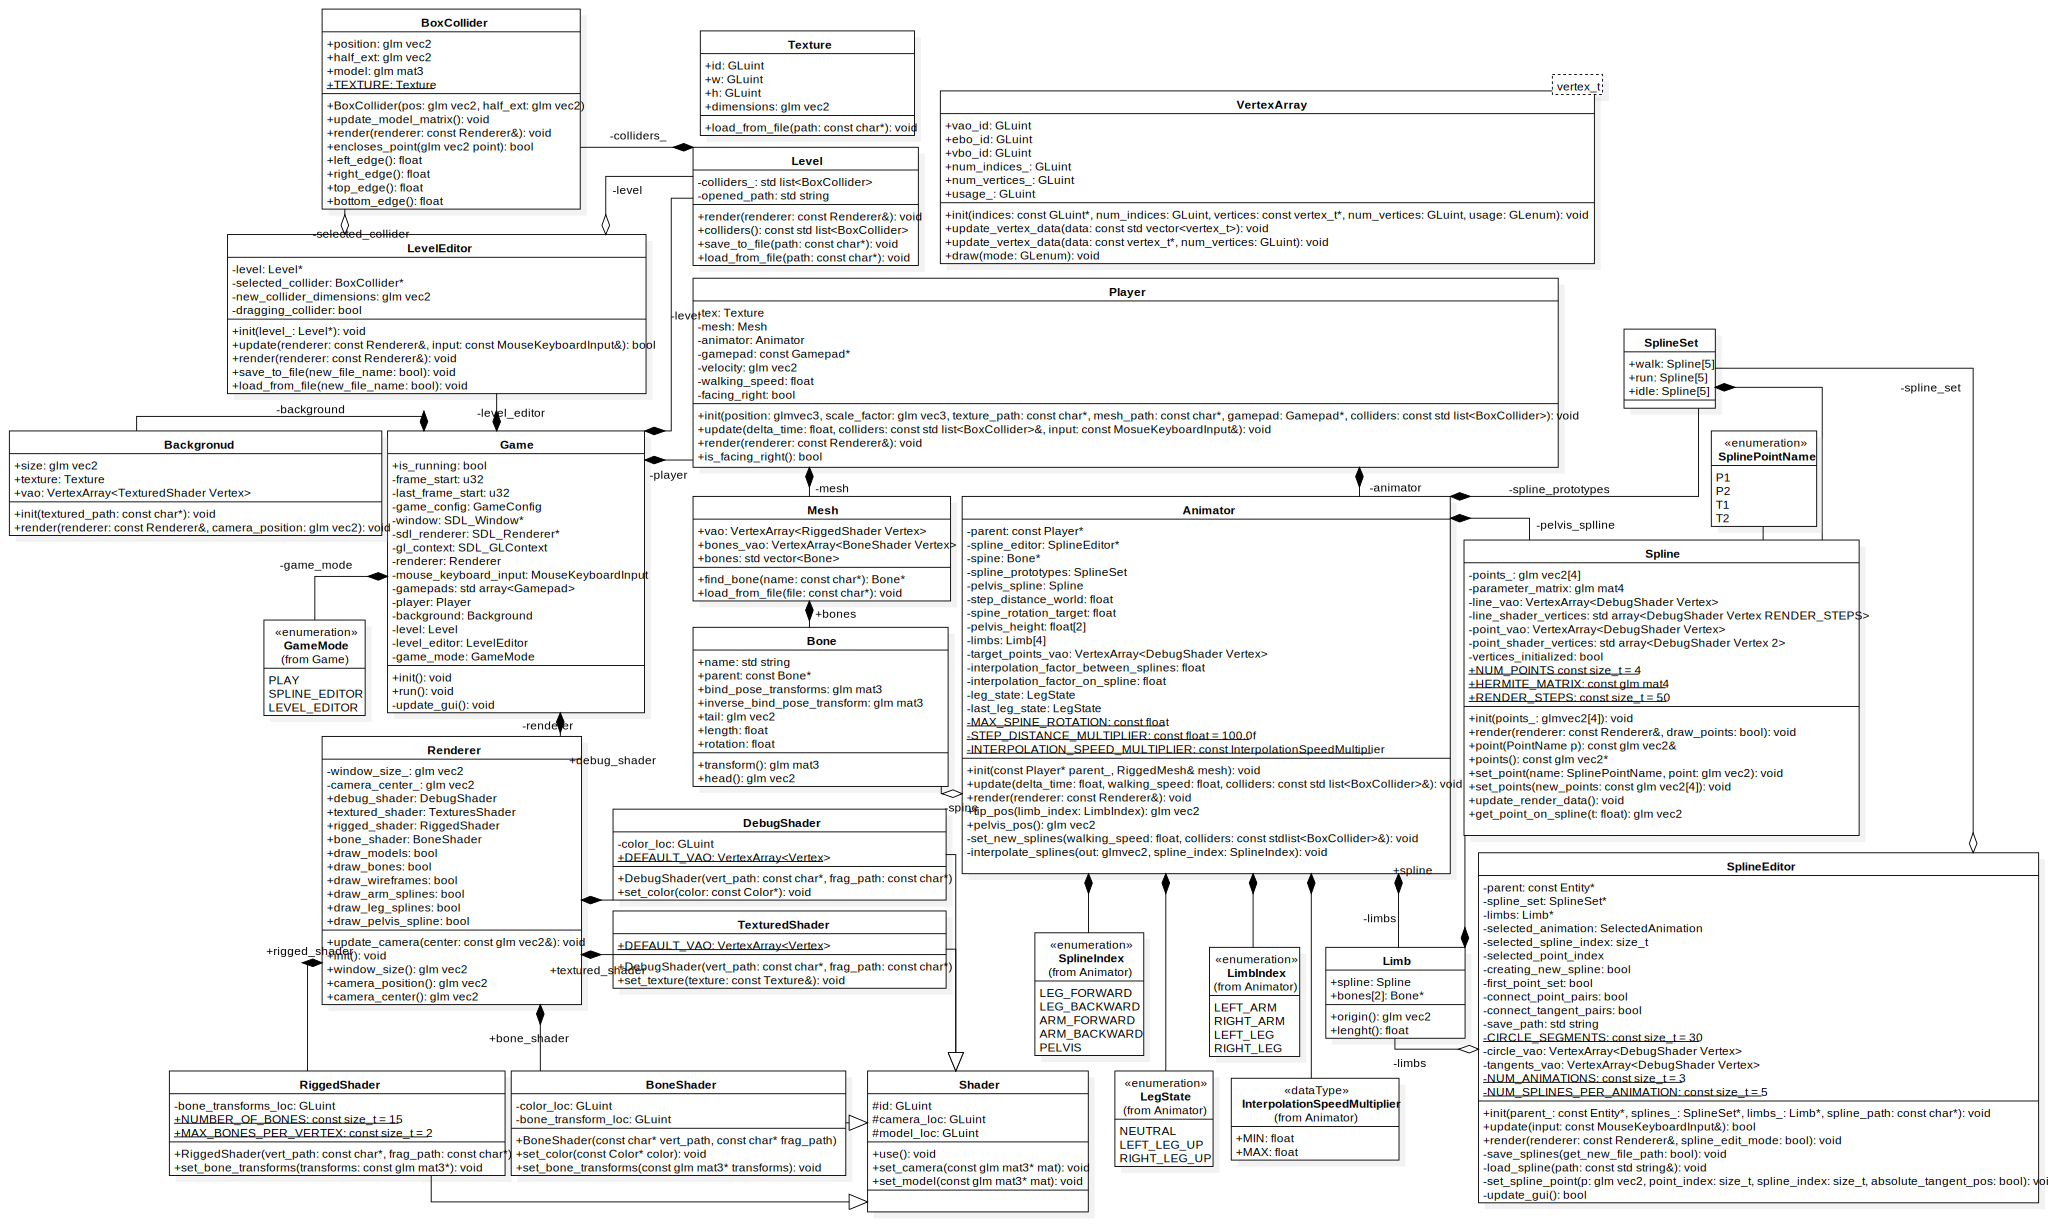
\includegraphics[width=\linewidth]{images/ClassDiagram.pdf}
        \caption{Objektdiagramm des gesamten Programms. Einige Klassen und Assoziationen wurden zur Verbesserung der Übersichtlichkeit ausgelassen.}
        \label{uml_classes}
    \end{figure}
\end{landscape}

\begin{figure}
    \centering
    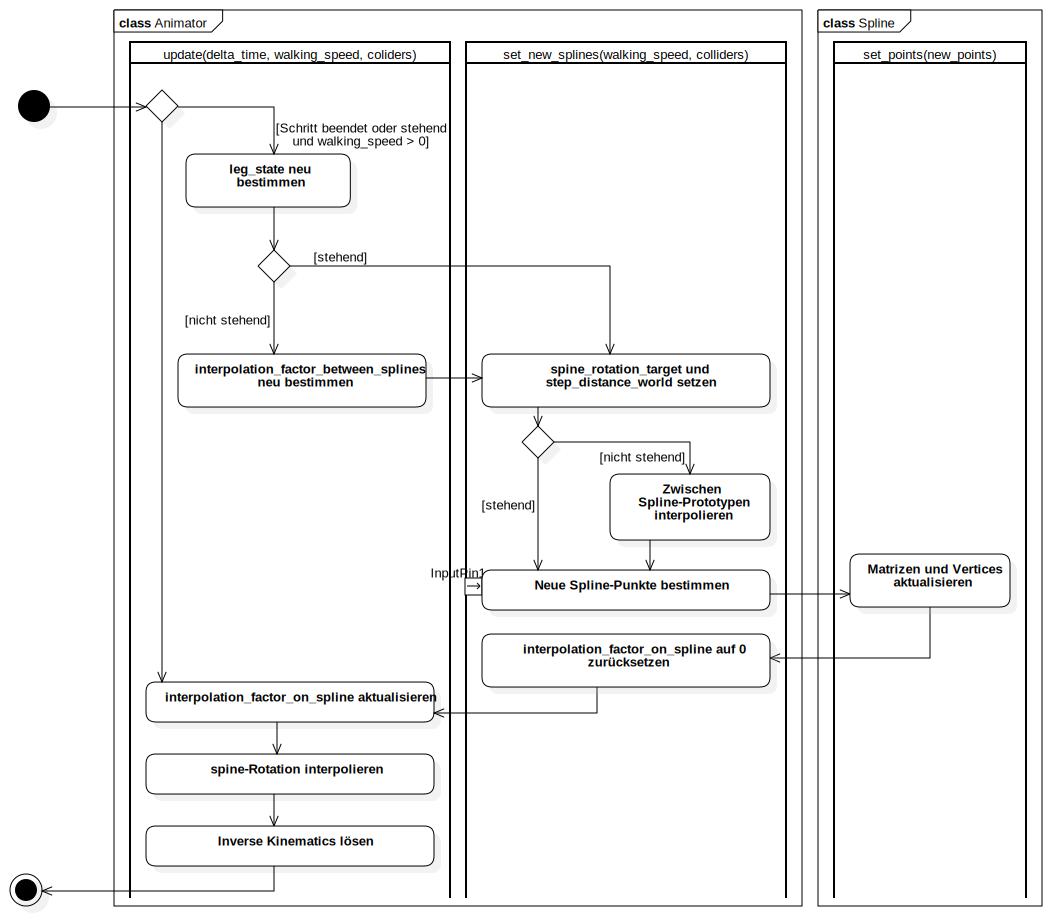
\includegraphics[width=\linewidth]{images/AnimatorActivity.pdf}
    \caption{Aktivitätsdiagramm des Animationsprozesses}
    \label{uml_activity}
\end{figure}